\chapter{Análise Bibliográfica sobre Deep Learning para Healthcare, por Caio Bernardon N. K. Massucato\label{chap:bibliometria:CaioMassucato}}

\section{Planejamento do estudo}

\textit{Deep Learning} para \textit{Healthcare} refere-se na utilização de \textit{deep learning}, um ramo da aprendizagem de máquina baseado na aprendizagem de representações de dados, para auxiliar nos cuidados de saúde das pessoas.

Algumas das representações de deep learning são inspiradas pelos avanços da neurociência e são vagamente baseadas na interpretação do processamento de informações e padrões de comunicação em um sistema nervoso, tais como codificação neural que tenta definir uma relação entre vários estímulos e as respostas neuronais associados no cérebro.

Com a popularização das inteligências artificiais, atualmente todas a aprendizagem de máquina vem tomando proporções muito grandes e consequentemente se tornou um tema muito discutido no mundo todo. Além disso, com esse avanço, IA começou a ser utilizada em cuidados para saúde.

Tendo como base o exposto acima, os pontos principais aqui abordados serão:
\begin{itemize}
    \item Onde o deep learning para healthcare está presente na sociedade?
    \item Quais os impactos dessas tecnologias que utilizam deep learning?
    \item Quais os dilemas éticos presentes nessas tecnologias?
\end{itemize}

\subsection{Uso do Bibliometrix e Biblioshiny}
Serão usadas a ferramenta e o \textit{workflow} proposto pelos autores do pacote Bibliometrix, conforme indica a figura ~\ref{fig:bibliometrix:workflow}.

\subsection{Limitações} A busca dos dados não foi extensa, dado o tempo utilizado para a mesma, além disso é um trabalho de principiante, não é esperada uma análise profunda.


\section{Coleta de dados\label{MASSA:coleta}}

A coleta de dados feita usando a base Web of Science (WoS) no dia 09 de Fevereiro de 2022, acessado por meio do Portal de Periódicos da CAPES

Foi usada a \textit{query} de busca ilustrada na listagem:

\lstinputlisting[numbers=left,basicstyle=\normalsize\ttfamily,caption={Query de busca: \textit{Deep Learning} para \textit{Healthcare}}]
{experiments/CaioMassucato/PesquisaBibliometrica/queries/query1.txt}

\subsection{Explicação para os termos de busca usados\label{sec:CaioMassucato:query}}

A busca utilizou cláusulas que retornassem registros relacionados a \textit{dep learning} utilizado em tecnologias de \textit{Healthcare}.

Os termos \textit{deep learning} e \textit{healthcare} com o conector AND trazem resultados apenas contendo ambos os conceitos., 

Foram obtidos 4305 registros com a \textit{query} utilizada. Na exportação, foi utilizado o formato de arquivo de texto sem formatação, com os 29 campos disponíveis e foram exportados 2000 dos 4305.

\section{Análise dos dados}

\subsection{Filtragem de registros}

Para a filtragem, removemos registros indesejados, supondo que o conhecimento de maior qualidade sobre o tema está nas publicações de artigos. Após a aplicação do filtro, 1143 registros foram mantidos no \textit{dataset} que servirá como objeto da análise.

\subsection{Análise descritiva do \textit{dataset} }

A seguir, é feita uma análise bibliométrica descritiva do \textit{dataset} utilizando a função \texttt{biblioAnalysis} do Bibliometrix, que realiza diversos cálculos para levantar as taxas apresentadas.

As informações mais gerais sobre o \textit{dataset} são as seguintes:
\begin{description}
    \item [\textit{Timespan}] Os artigos filtrados foram publicados entre 2004 e 2022.
    \item [\textit{Sources (Journals, Books, etc)}] São 445 fontes de informação que publicaram os artigos recuperados no \textit{dataset}.
    \item [\textit{Average years from publication}] A média do tempo de publicação dos artigos no \textit{dataset} é de 1,92 anos.
    \item [\textit{Average citations per documents}] Cada artigo no \textit{dataset} foi citado, em média 15,14 vezes.
    \item [\textit{Average citations per year per doc}] Após publicado, cada um dos artigos foi citado, em média, 3.925 vezes por ano.
    \item [\textit{References}] O \textit{dataset} contém 40.227 referências citadas.
    \item [\textit{Keywords Plus (ID)}] 1.689 distintas palavras-chave do tipo Keywords Plus (ID) foram encontradas no \textit{dataset}.
    \item [\textit{Author's Keywords (DE)}] 2.964 distintas palavras-chave indicadas pelos autores foram encontradas no \textit{dataset} .
    \item [\textit{Authors}] 5.967 autores distintos foram encontrados no \textit{dataset} .
    \item [\textit{Author Appearances}] 7.243.
    \item [\textit{Authors of single-authored documents}] Dentre os 5.967 autores encontrados, 26 deles editaram artigos individualmente, isso é, sem co-autores.
    \item [\textit{Authors of multi-authored documents}] Dentre os 5.967 distintos (nomes de) autores encontrados, 5.941 deles editaram artigos com um ou mais co-autores"
    \item [\textit{Single-authored documents}] Dentre os 1.143 documentos presentes no \textit{dataset}, 27 foram escritos por um único autor, e os restantes foram elaborados em co-autoria.
    \item [\textit{Documents per Author}] Dentre os 5.967 autores, cada um publicou em média 0,192 artigos.
    \item [\textit{Authors per Document}] Cada um dos 1.143 documentos presentes no \textit{dataset} foi autorado com 5,22 autores em média.
    \item [\textit{Co-Authors per Documents}] Existe em média 6,34 co-autores por documento.
    \item [\textit{Collaboration Index}] O index de colaboração é 5,32
\end{description}

\subsection{Evolução da Produção Científica}

\begin{figure}
    \centering
    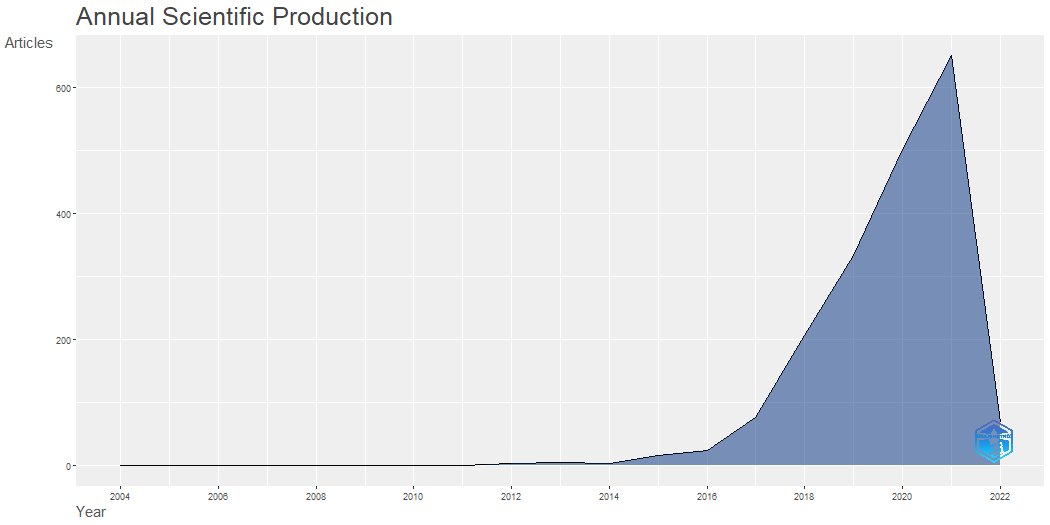
\includegraphics[width=1\textwidth]{experiments/CaioMassucato/PesquisaBibliometrica/DeepLearningHC/AnnualScientificProduction-2022-02-10.png}
    \caption{Evolução da produção científica no \textit{dataset}}
    \label{fig:evol:anual:DEEPLEARNINGHC@CaioMassucato}
\end{figure}

A figura \ref{fig:evol:anual:DEEPLEARNINGHC@CaioMassucato} mostra a relação da produção científica mundial a respeito do tema pelo tempo, de acordo com o \textit{dataset}. O assunto possui notoriedade desde 2013, com os maiores crescimentos nos anos de 2007 e 2018, atingindo o pico no ano de 2021. 

O \textit{Annual Growth Rate} do \textit{dataset} é de 35.03\%.

\subsection{Interpretação do Crescimento} A taxa de crescimento é muito alta quando comparada com de outros temas no âmbito da produção científica. Os números mostram grande crescimento do tema nos ultimos anos, o que é esperado devido ao crescente uso das inteligências artificiais no dia-a-dia das pessoas, em casas intelignetes, \textit{wearables} e outros.

\subsection{Evolução das Citações}

\begin{figure}
    \centering
    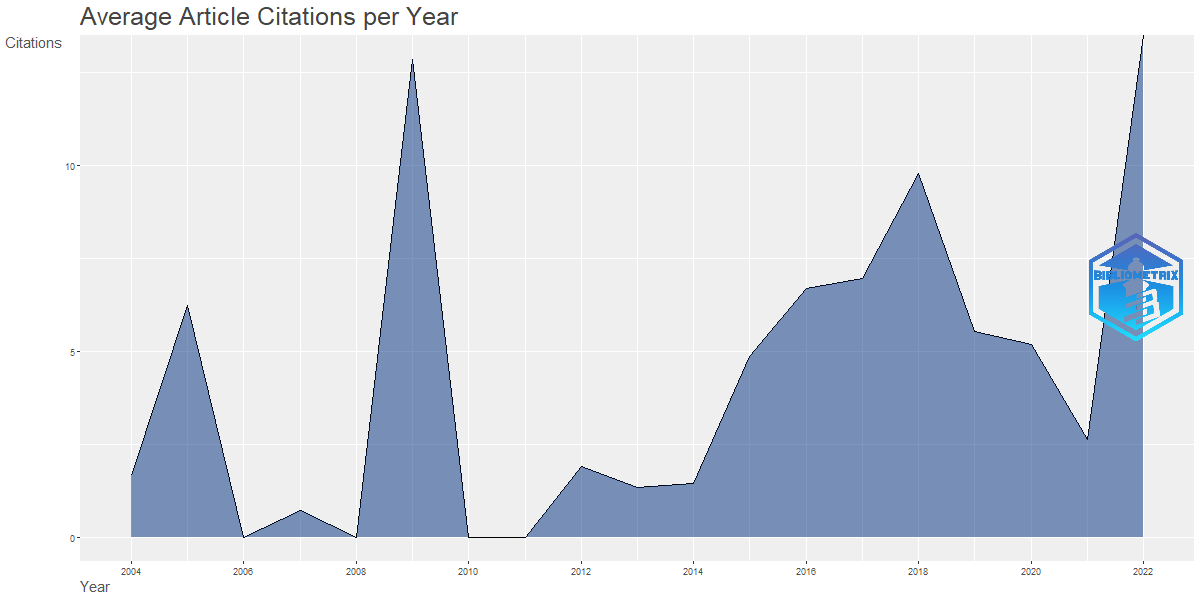
\includegraphics[angle=0,width=1\textwidth]{experiments/CaioMassucato/PesquisaBibliometrica/DeepLearningHC/AverageArticleCitationPerYear-2022-02-10.png}
    \caption{Evolução das citações ao \textit{dataset}.}
    \label{fig:evol:anual:citacoes:DEEPLEARNINGHC@CaioMassucato}
\end{figure}

A figura \ref{fig:evol:anual:citacoes:DEEPLEARNINGHC@CaioMassucato} apresenta a evolução da média de citações aos artigos do \textit{dataset}. Os números para a média de citações é um tanto incerto.

\subsection{Interpretação das Citações}
O gráfico mostra que o tema precisa de um pouco mais de tempo no meio científico para que o número de citações atinja uma forma estável.

\subsection{\textit{Three-Field Plots (Sankey diagram)}}

As \textit{Three-Field Plots (Sankey diagram)} (plotagens do tipo ``Três Campos'') correlacionam três conjuntos de atributos em busca das afinidades encontradas no \textit{dataset}. Assim, são demonstrados os principais fluxos entre diferentes conjuntos.

\begin{figure}
    \centering
    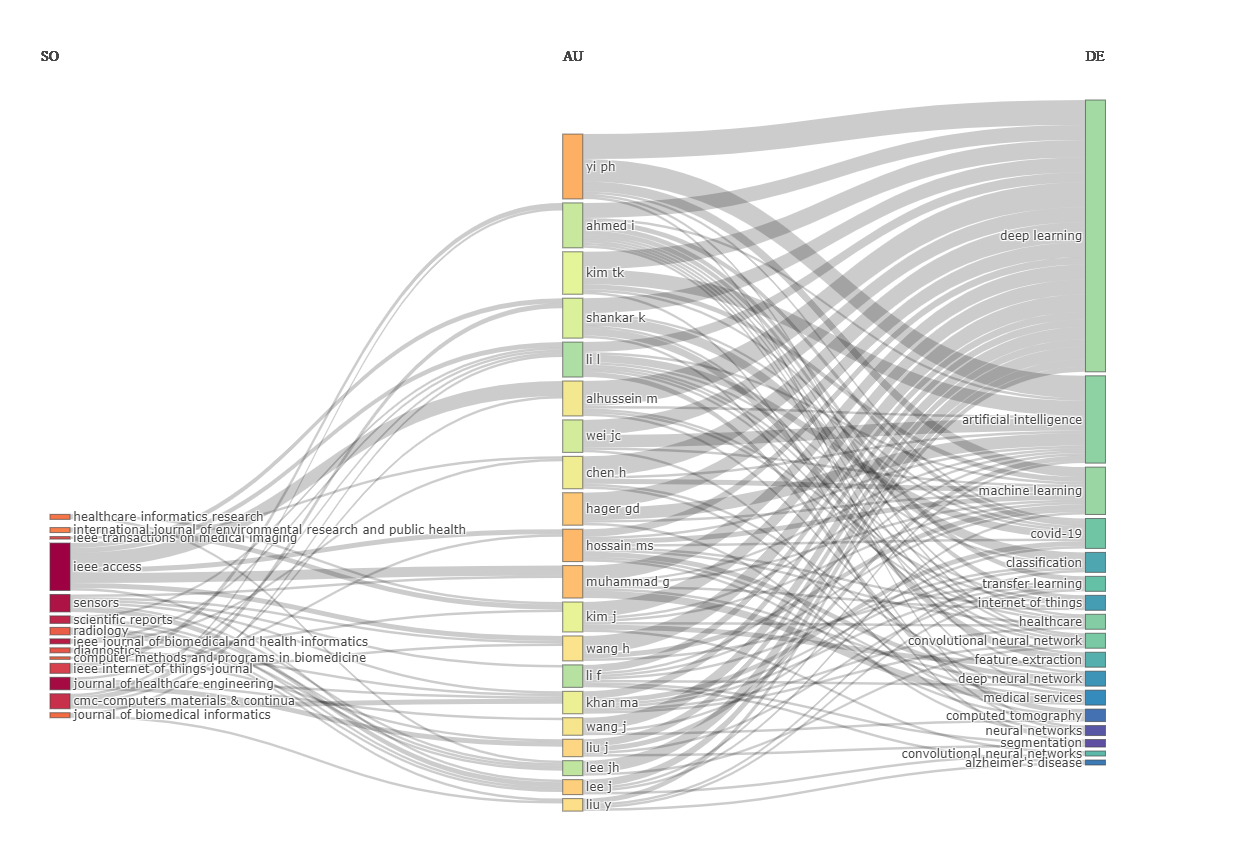
\includegraphics[width=1\textwidth]{experiments/CaioMassucato/PesquisaBibliometrica/DeepLearningHC/threeFields.png}
    \caption{Plotagem ``Três Campos'' (Sankey plot)}
    \label{fig:threeFields:DEEPLEARNINGHC@CaioMassucato}
\end{figure}

A figura \ref{fig:threeFields:DEEPLEARNINGHC@CaioMassucato} apresenta a plotagem do tipo ``Três Campos'' realizada sobre os dados presentes no \textit{dataset}, que relaciona:  os Autores mais relevantes (AU), as Citações mais frequentes (CR), e as Palavras-Chave mais frequentes nos registros.

\subsection{Interpretação da figura \ref{fig:threeFields:DEEPLEARNINGHC@CaioMassucato}}
A maioria das publicações possui relação com a IEEE, que mostra a influencia e a investida do instituto nas pesquisas sobre o tema. Além disso, podemos notar a relação entre as diversas áreas da inteligência artificial e da aprendizagem de máquina pelas palavras chave mais frequentes, onde aparecem \textit{artificial intelligence}, \textit{machine learning}, \textit{convolutional neural networks} e outros.

Além disso, pode-se notar que "covid-19" é a 4ª palavra-chave mais utilizada dentre os autores, o que pode explicar também o pico que o assunto obteve durante o ano de 2021, mostrado na figura \ref{fig:evol:anual:DEEPLEARNINGHC@CaioMassucato}.

\section{Refinamento da Coleta de Dados}

Não foi observado nenhum motivo para haver refinamento da coleta de dados, os dados retornados aparentemente estão de acordo com o que foi esperado no momento da busca.

\section{Nova Análise dos Dados}

\subsection{Nova filtragem de registros}

\subsection{Análise descritiva do \textit{dataset} refinado}